\documentclass{article}

    \usepackage[T1]{fontenc}
    \usepackage[utf8]{inputenc}
    \usepackage{float}
    \usepackage[french]{babel}
    \usepackage[margin=.8in]{geometry}
    \usepackage{amssymb}
    \usepackage{amsmath}  
    \usepackage{mathtools}
    \usepackage{listings}
    \usepackage{graphicx}
    \usepackage[hidelinks]{hyperref}
    \usepackage{calrsfs}
    
    \begin{document}
        
        \title{Projet 1 : transformation du plan}
        \author{Nathan Soufflet}
    
        \maketitle
        \pagenumbering{gobble}
        \newpage
    
        \section{Etude de la fonction $f(z) = z^{2}$}
    
        \subsection{}

        Soient $A(1, -1)$ et $B(1, 1)$ les points d'affixes respectives $z_A = 1 - i$, $z_B = 1 + i$

        Le segment $[A, B]$ peut être paramétré comme suit :

        \begin{align*}
            \gamma : [0, 1] \to \mathbb{C} \\ t \mapsto z_A + 2ti
        \end{align*}

        d'où $f(\gamma(t)) = (z_A + 2ti)^{2} = (1 - i + 2ti)^{2} = 4t(1 - t) + i(4t - 2)$

        Soit $f(\gamma(t)) = x + iy$ avec $(x, y) \in \mathbb{R}^{2}$, alors : 
    
        \begin{equation*}
            \left \{
            \begin{aligned}
              &x = 4t(1 - t) \\
              &y = 4t - 2
            \end{aligned} \right.
        \end{equation*} 

          $\Leftrightarrow x = (y + 2)(1 - \frac{y + 2}{4})$ 
          soit : 
          $$\fbox{$x = -\frac{1}{4} y^2 + 1$}$$

          pour $y \in [-2, 2]$, il s'agit donc bien d'une portion de parabole.

          \begin{figure}[ht!]
            \centering
            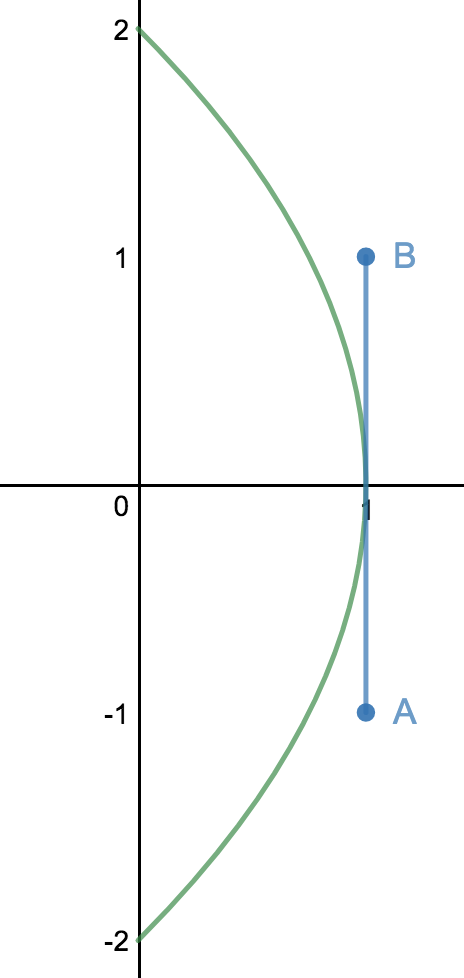
\includegraphics[height=0.5\textwidth]{figures/segAB.png}
            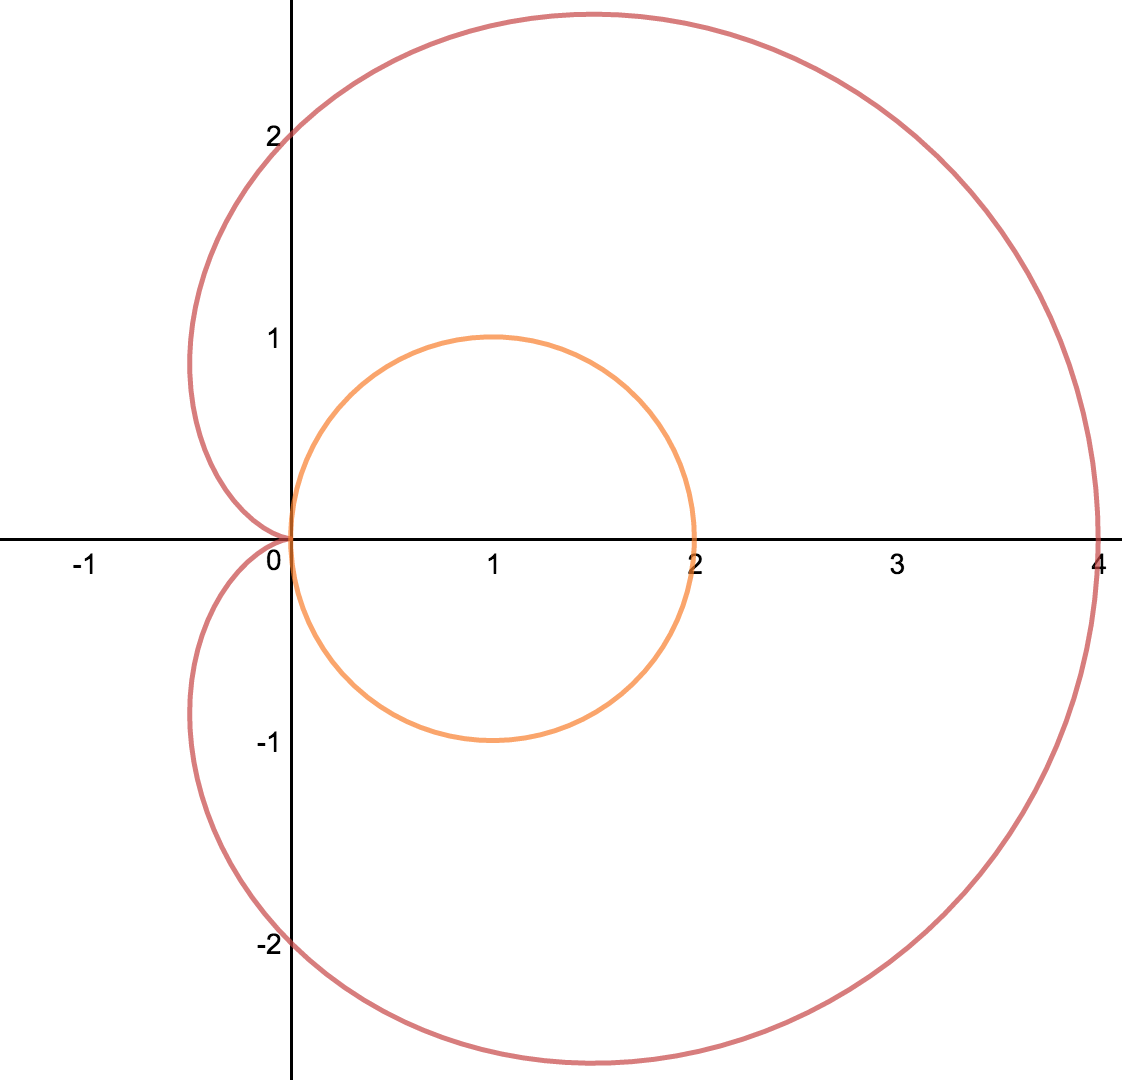
\includegraphics[height=0.5\textwidth]{figures/cardioide.png}
            \caption{Segment $[A, B]$, cercle $\mathcal{C}$ et leur image par $f$}
          \end{figure}

          \subsection{}

          Soit $\mathcal{C}$ le cercle de centre $C(1, 0)$ et de rayon 1.

          Une parametrisation de $\mathcal{C}$ est :

        \begin{align*}
            \gamma : [0, 2\pi] \to \mathbb{C} \\ t \mapsto e^{it} + 1
        \end{align*}

        on a alors $f(\gamma(t)) = (e^{it} + 1)^{2} = e^{2it} + 2e^{it} + 1$

        d'où : 

        \begin{equation*}
            \left \{
            \begin{aligned}
              &x = 1 + \cos(2t) + 2\cos(t) \\
              &y = \sin(2t) + 2\sin(t)
            \end{aligned} \right.
        \end{equation*} 
        
        en utilisant les identités de l'angle double, on obtient :

        \begin{equation*}
            \left \{
            \begin{aligned}
              &x = 2(1 + \cos(t))\cos(t) \\
              &y = 2(1 + \cos(t))\sin(t)
            \end{aligned} \right.
        \end{equation*}

        L'écriture polaire suit directement : 

        $$\fbox{$\rho(\theta) = 2(1 + \cos(\theta))$}$$

        \section{Transformations conformes}

        \subsection{Translation}

        Expression d'une translation par $\vec{v}(a, b)$ dans le plan complexe : $\fbox{$g(z) = z + a + ib$}$

        $g(z)$ est une somme de deux fonctions entières : $z \mapsto z$ et $z \mapsto a + ib$ et est
        donc également entière.

        \begin{figure}[ht!]
            \centering
            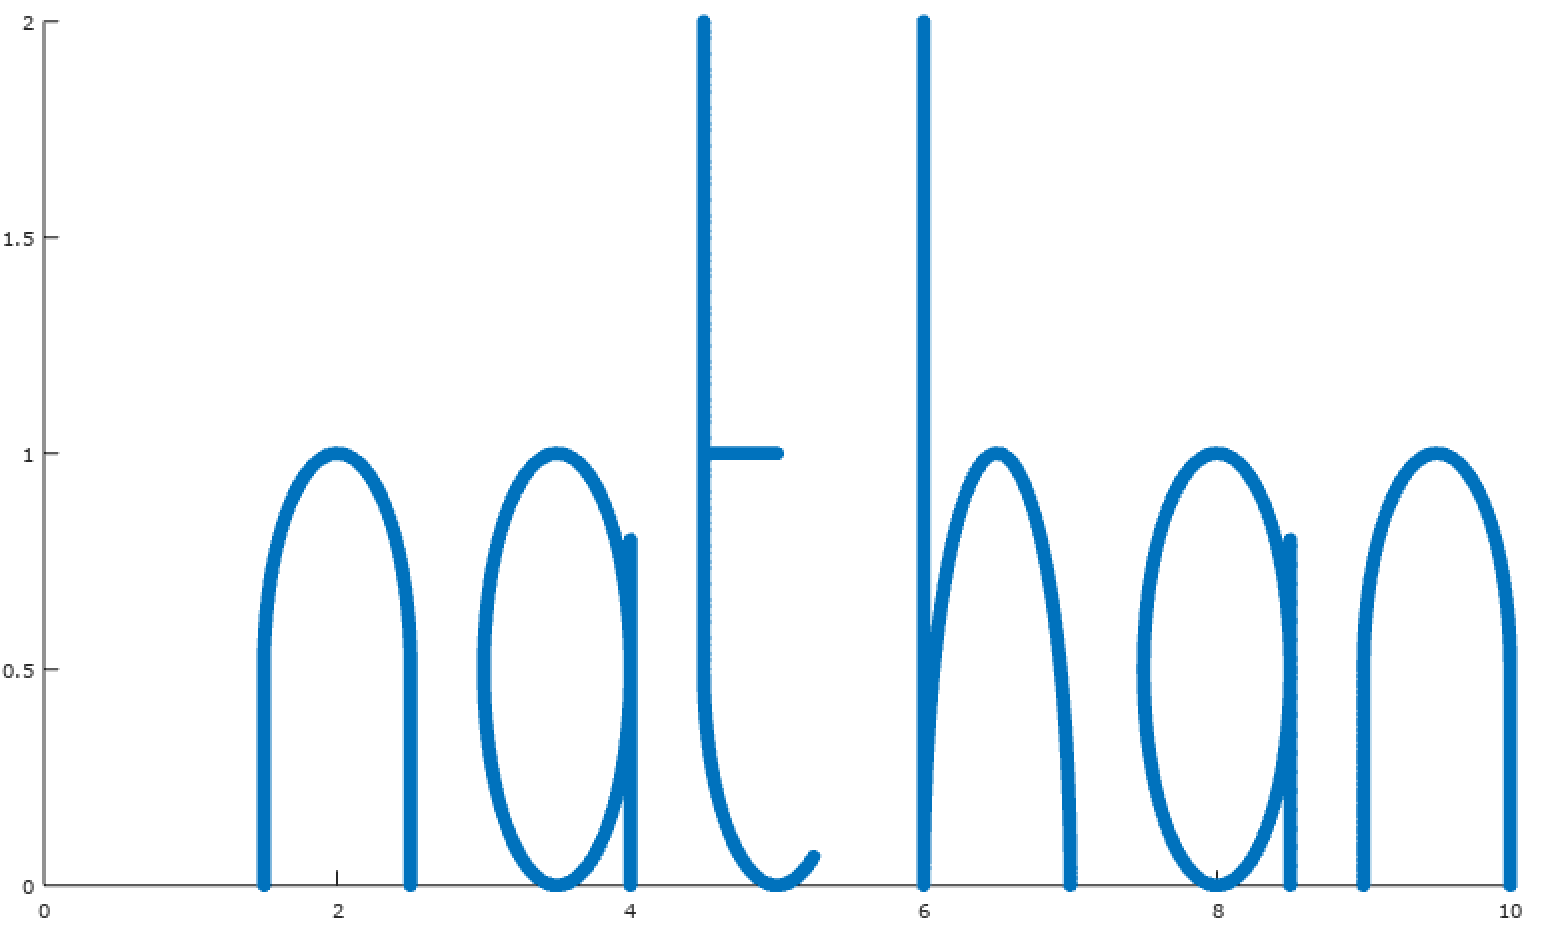
\includegraphics[height=0.3\textwidth]{figures/name.png}
            \caption{Mon prénom composé des lettres de alphabet.m}
          \end{figure}

    \subsection{Fonction holomorphe quelconque}

    \begin{figure}[ht!]
        \centering
        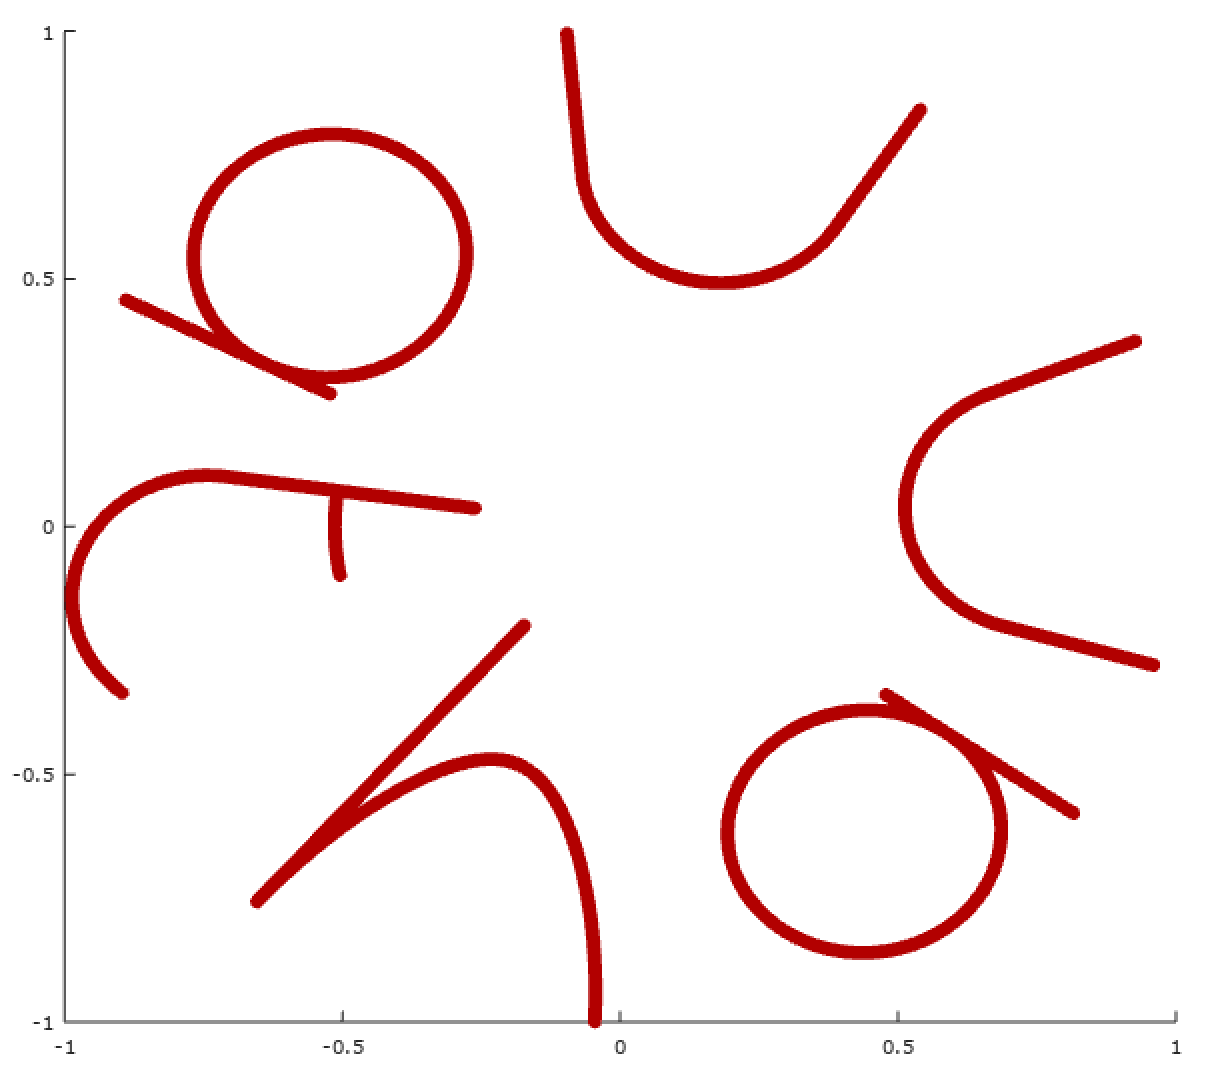
\includegraphics[height=0.32\textwidth]{figures/name2.png}
        \caption{Image de mon prénom par $z \mapsto exp(\frac{2iz}{3})$}
      \end{figure}


      \subsection{Rotation}

      Expression d'une rotation de centre $M_{0}(z_{0})$ et d'argument $\theta$ : 
      $\fbox{$g(z) = e^{i\theta}(z - z_{0}) + z_{0}$}$

      $g(z)$ peut s'écrire $g(z') = az' + z_{0}$, avec $a = e^{i\theta}$ et $z' = z - z_{0}$, il s'agit
      ainsi d'une fonction affine donc entière.

      \begin{figure}[ht!]
        \centering
        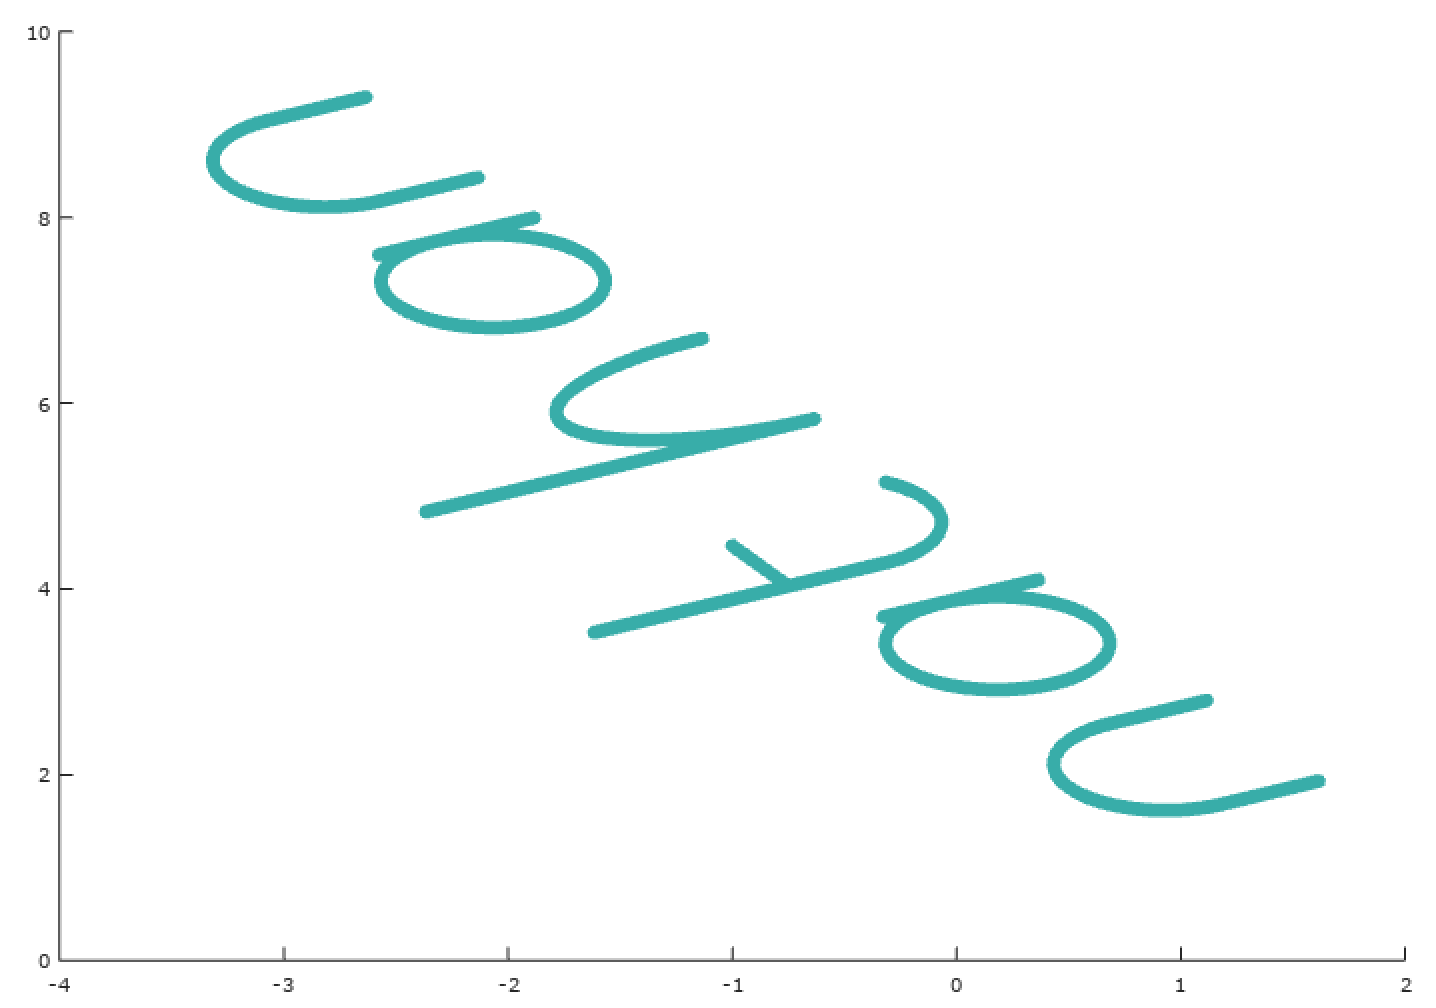
\includegraphics[height=0.32\textwidth]{figures/rotation2.png}
        \caption{Rotation de mon prénom avec $z_{0} = 1 + i$ et $\theta = \frac{2 \pi}{3}$}
      \end{figure}

      \subsection{Homothétie}

      Expression d'une homothétie de centre $M_{0}(z_{0})$ et de rapport $k \in \mathbb{R}$ : 
      $\fbox{$g(z) = k(z - z_{0}) + z_{0}$}$

      $g(z)$ est une fonction affine donc entière.

      \begin{figure}[ht!]
        \centering
        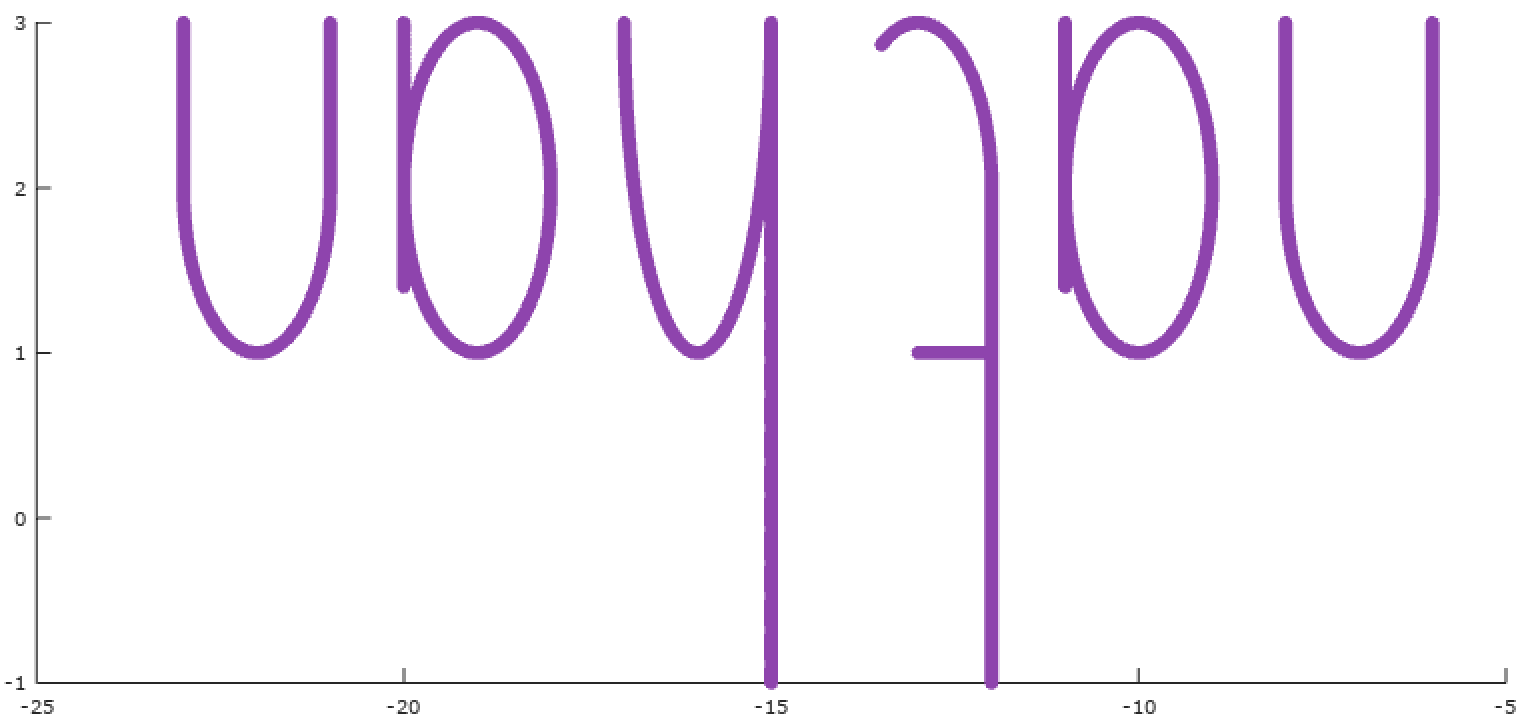
\includegraphics[height=0.32\textwidth]{figures/homothetie.png}
        \caption{Homothétie de mon prénom avec $z_{0} = i - 1$ et $k = -2$}
      \end{figure}

      Soient $f, g$ et $h$ telles que :

      \begin{equation*}
        \left \{
        \begin{aligned}
          &f(z) = z + 2 + 2i \\
          &g(z) = e^{i\frac{\pi}{3}}z \\
          &h(z) = 2z
        \end{aligned} \right.
    \end{equation*} 

    $h \circ g \circ f$ est la composition de fonctions entières, et est don également entière. \\

    L'ordre dans lequel sont effectuées des rotations, translations et homotheties importe, ce qui s'exprime par la non-commutativité 
    de la composition de ces transformations :

    $$h \circ g \circ f = 2e^{i\frac{\pi}{3}}(z + 2 + 2i) \neq f \circ g \circ h = 2e^{i\frac{\pi}{3}}z + 2 + 2i$$

    \subsection{Symétrie centrale}

    Une symétrie centrale correspond à une rotation d'un demi-tour autour d'un point.
    On en déduit une expression d'une symétrie centrale de centre $M_{0}(z_{0})$ : 
    $\fbox{$g(z) = e^{i\pi}(z - z_{0}) + z_{0} = 2z_{0} - z$}$

    $g(z)$ étant une rotation, il s'agit d'une fonction entière.

    \begin{figure}[ht!]
        \centering
        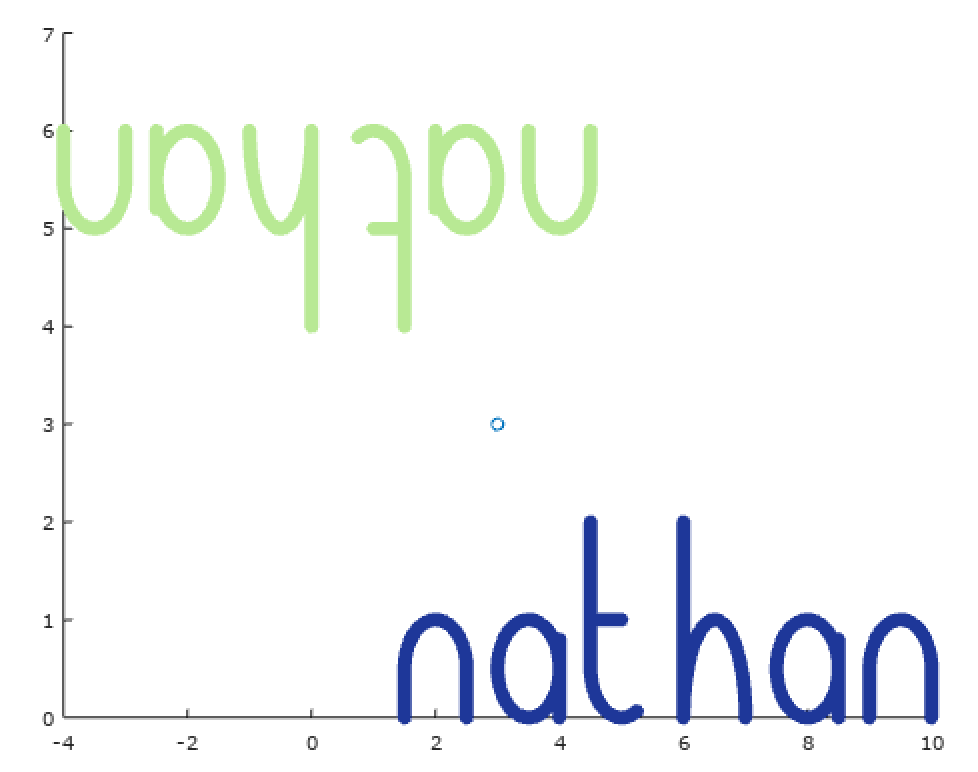
\includegraphics[height=0.32\textwidth]{figures/sym_centrale.png}
        \caption{Symétrie centrale de centre d'affixe $z_{0} = 3 + 3i$}
    \end{figure}


      Soient $u$ et $v$ deux fonctions de $\mathbb{C} \to \mathbb{C}$ telles que :

      \begin{equation*}
        \left \{
        \begin{aligned}
          &u(z) = e^{i\pi}z = -z \\
          &v(z) = z + 2z_{0}
        \end{aligned} \right.
    \end{equation*} 

    Par identification, $u$ correspond à une rotation et $v$ à une translation, avec :
    
    $$\fbox{$(v \circ u)(z) = g(z)$}$$
    
    la symmetrie centrale est donc la composition d'une rotation de $\pi$ radians suivie d'une 
    translation de $2z_{0}$.


    \subsection{Symétrie axiale}

    Expression d'une symétrie d'axe $x = 0$ : $\fbox{$g(z) = \overline{z}$}$ \\

    $\forall z \in \mathbb{C}, \frac{\partial g(z)}{\partial \overline{z}} = 1 \neq 0$ donc $g(z)$ n'est holomorphe
    nulle part, en effet une symétrie axiale ne conserve pas l'orientation des angles (sens inversé).

    \begin{figure}[ht!]
        \centering
        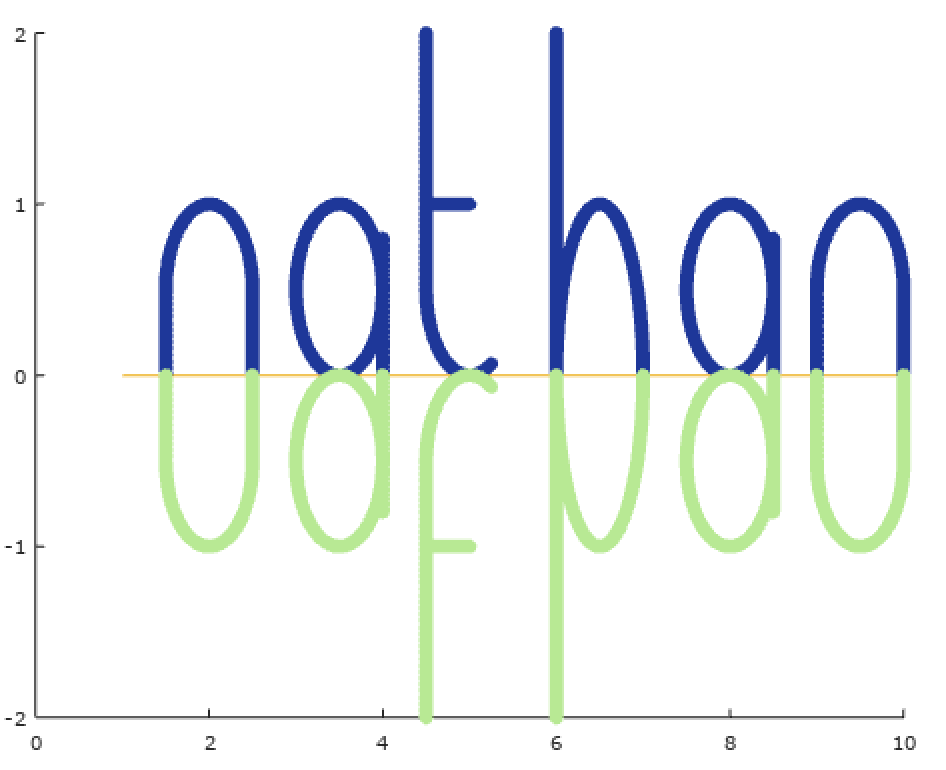
\includegraphics[height=0.32\textwidth]{figures/sym_axiale.png}
        \caption{Symétrie axiale selon l'axe des abscisses}
    \end{figure}

    \subsection{Symétrie axiale (démonstration)}

    - L'ensemble $\{z_{0} + (1 + a)\alpha, \alpha \in \mathbb{R}\}$ représente l'axe $(\Delta_{0})$. \\
    
    - Soit $f(z) = a\overline{(z - z_0)} + z_0$ et 
    $\alpha \in \mathbb{R}$, avec $a = e^{i\theta} = \cos(\theta) + i\sin(\theta)$ \\
    \
    d'où 
    $f(z_{0} + (1 + a)\alpha) = a\overline{(1 + a)\alpha} + z_0 = \alpha [cos(\theta) + i\sin(\theta)][1 + \cos(\theta) - i\sin(\theta)] + z_0$ \\
    \
    finalement
    $f(z_{0} + (1 + a)\alpha) = \alpha [\cos(\theta) + i\sin(\theta) + \cos^2(\theta) + \sin^2(\theta)] + z_0 =  z_0 + (1 + a)\alpha$ \\
    
    On a donc bien $\fbox{$f(z_{0} + (1 + a)\alpha) = z_{0} + (1 + a)\alpha, \forall \alpha \in \mathbb{R} \Leftrightarrow f(\Delta_0) = \Delta_0$}$\\

    On vient ainsi de démontrer que l'axe $(\Delta_0)$ est un ensemble d'invariants de $f$ et correspond donc à l'axe
    de symétrie de la transformation $f(z)$.\\

    - En utilisant la formule d'Euler : $\fbox{$2\cos(\frac{\theta}{2}) e^{i\frac{\theta}{2}} =
     (e^{i\frac{\theta}{2}} + e^{-i\frac{\theta}{2}})e^{i\frac{\theta}{2}} = 1 + e^{i\theta} = 1 + a$}$\\

     - En utilisant l'égalité précedente, on a : \\

     $$z_0 + \frac{a + 1}{4 \cos(\frac{\theta}{2})} (e^{i\frac{\theta}{2}} (\overline{z - z_0}) + 
     e^{-i\frac{\theta}{2}} (z - z_0)) 
     = 
     z_0 + \frac{2cos(\frac{\theta}{2}) e^{i\frac{\theta}{2}}}{4 \cos(\frac{\theta}{2})} (e^{i\frac{\theta}{2}} (\overline{z - z_0}) + 
     e^{-i\frac{\theta}{2}} (z - z_0))$$

     $$ = z_0 + \frac{e^{i\frac{\theta}{2}}}{2} [e^{i\frac{\theta}{2}}(\overline{z - z0}) + e^{-i\frac{\theta}{2}} (z_0 - z)]
     =
     \frac{e^{i\frac{\theta}{2}} (\overline{z - z_0}) + z_0 + z}{2}
     =
     \frac{f(z) + z}{2}
     $$\\
     
     On a donc bien $\fbox{$\frac{f(z) + z}{2} = z_0 + \frac{a + 1}{4 \cos(\frac{\theta}{2})} (e^{i\frac{\theta}{2}} (\overline{z - z_0}) + 
     e^{-i\frac{\theta}{2}} (z - z_0)) $}$\\


     - Soit $\alpha_m$ tel que : 
     
     $$\alpha_m = \frac{e^{i\frac{\theta}{2}} (\overline{z - z_0}) + e^{-i\frac{\theta}{2}} (z - z_0)}{4 \cos(\frac{\theta}{2})}$$
     où $z - z_0 = x + iy$ avec $(x, y) \in \mathbb{R}^{2}$\\
     
     On a alors : 
     $$\alpha_m = \frac{e^{i\frac{\theta}{2}} (x + iy) + e^{-i\frac{\theta}{2}} (x - iy)}{4 \cos(\frac{\theta}{2})}
     =
     \frac{x(e^{i\frac{\theta}{2}} + e^{-i\frac{\theta}{2}}) +iy(e^{i\frac{\theta}{2}} - e^{-i\frac{\theta}{2}})}{4 \cos(\frac{\theta}{2})}
     $$

     En utilisant l'écriture complexe de $\cos$ et $\sin$, on obtient $\forall \theta \not \equiv \frac{\pi}{2}\ (\textrm{mod}\ 2\pi)$

     $$\alpha_m = \frac{x\cos(\frac{\theta}{2}) + y\sin(\frac{\theta}{2})}{2 \cos(\frac{\theta}{2})}
     =
     \frac{1}{2} (x + y \tan{\frac{\theta}{2})} \in \mathbb{R}$$

     Notons $M(z), M'(f(z))$ et $M_m$ milieu du segment $[M, M']$ d'affixe $\frac{f(z) + z}{2}$, ce qui permet d'écrire : 

     $$(1) : \forall \theta \in \mathbb{R} - \{\frac{\pi}{2} + 2\pi\mathbb{Z}\}, \ \exists \alpha = \alpha_m \in \mathbb{R}
     \mid z_0 + (1 + a) \alpha = \frac{f(z) + z}{2} \Rightarrow \fbox{$M_m \in (\Delta_0)$}$$\\

    - Soient $\vec{u}$ et $\vec{v}$ deux vecteurs d'affixes respectives $z = x + iy$ et $z' = x' + iy'$, avec $(x, y, x', y') \in \mathbb{R}^{4}$, on a alors : \\

    $$z \overline{z'} + z' \overline{z} = (x + iy) (x' - iy') + (x' + iy') (x - iy)$$

    $$ = (xx' - ixy' + ix'y + yy') + (xx' - ix'y + ixy' + yy') = 2(xx' + yy')$$

    On en déduit :

    $$\fbox{$z \overline{z'} + z' \overline{z} = 2(\vec{u}.\vec{v}) = 0 \Leftrightarrow \vec{u}.\vec{v} = 0 
    \Leftrightarrow \vec{u} \perp \vec{v}$}$$

    \newpage

    - Soient $\vec{u}$ et $\vec{v}$ des vecteurs d'affixes respectives $f(z) - z$ et $a + 1$, d'après l'équivalence précédente, on a : 

    $$\vec{u} \perp \vec{v} \Leftrightarrow (\overline{a} + 1) (f(z) - z) + (a + 1) (\overline{f(z) - z}) = 0$$

    $$\Leftrightarrow (\overline{a} + 1) (a(\overline{z - z_0}) + z_0 - z) + (a + 1) (a(z - z_0) + \overline{z_0 - z}) = 0$$

    Or $a = e^{i\theta}$ d'où : 

    \begin{equation*}
        \left \{
        \begin{aligned}
          &a(\overline{a} + 1) = (\cos{\theta} + i\sin{\theta}) (1 + \cos{\theta} - i\sin{\theta}) = 1 + \cos{\theta} + i\sin{\theta} = a + 1 \\
          &\overline{a}(a + 1) = (\cos{\theta} - i\sin{\theta}) (1 + \cos{\theta} + i\sin{\theta}) = 1 + \cos{\theta} - i\sin{\theta} = \overline{a} + 1
        \end{aligned} \right.
    \end{equation*} 

    On a donc :

    $$\vec{u} \perp \vec{v} \Leftrightarrow (a + 1) (\overline{z - z_0} + \overline{z_0 - z}) 
    +
     (\overline{a} + 1) (z_0 - z + z - z_0) = 0$$

    Finalement,

    $$\forall z \in \mathbb{C}, \ \vec{u} \perp \vec{v}$$

    De plus, le segment $[MM']$ et la droite $(\Delta_0)$ ont pour vecteur directeur (resp.) $\vec{u}$ et $\vec{v}$, 
    on en déduit :

    $$\fbox{$(2) : [MM'] \perp (\Delta_0)$}$$

    - D'après $(1)$ et $(2)$ on a donc (pour toute droite $(\Delta_0)$ non verticale) :

    $$\fbox{$\forall M(z \in \mathbb{C}), \ M_m \in (\Delta_0) \land [MM'] \perp (\Delta_0)$}$$

    $(\Delta_0)$ est donc la médiatrice du segment $[MM']$. \\

    
    Ainsi, la fonction $f$ transforme un point $M(z)$ 
    en $M'(f(z))$ tel que la droite $(\Delta_0)$ passant par $z_0$ et de vecteur directeur d'affixe $1 + a$ soit 
    la médiatrice du segment $[MM']$. \\ 
    \underline{La définition algébrique est donc cohérente avec la définition géométrique.}


    \end{document}